\chapter{Introduction}
\begin{multicols}{2}
      [\section{Project Background}]
      In today's rapidly evolving digital landscape, cybersecurity remains a paramount concern for organizations
      across all industries. With the proliferation of sophisticated cyber threats and the increasing complexity of
      \acrshort{it} infrastructures, business are constantly seeking new and innovative ways to protect their
      digital assets and fortify their defences and safeguard sensitive data. In this pursuit, cybersecurity
      consultant firms have emerged as a critical ally for organizations, providing expert guidance and support in
      the development and implementation of robust cybersecurity strategies, playing a pivotal role in offering
      expertise and guidance to help organizations navigate the intricate realm of cybersecurity.

      One of the key strategies employed by cybersecurity consultants is the integration of third-party security
      \gls{API}s into their arsenal of tools and technologies. These \acrshort{api}s provide invaluable
      functionalities, ranging from vulnerability assessment and security scans to device health monitoring and
      threat intelligence analysis by \acrshort{ai}. By leveraging these \acrshort{api}s, cybersecurity consultants
      can enhance their capabilities and provide a more comprehensive and effective security solution to their
      clients, streamline their operations, provide clients with robust, proactive security measurers, and improve
      their overall service delivery.

      SentinelOne....

      \section{The Company and the QaaS App}
      \acrshort{qict} \acrshort{bv}, is a small cybersecurity consultancy based in Emmen, northeast of the
      Netherlands. It recognizes the critical importance of proactive \acrshort{api} monitoring in safeguarding
      its clients' digital assets. Their customers are \acrshort{sme} companies with employees ranging from 1 to 100.
      \acrshort{qict} is therefore asked to monitor their clients' devices and ensuring the overall security of
      their systems, \acrshort{it} infrastructure, and digital assets. They typically engage in various activities,
      including:
      \begin{itemize}
            \item \textbf{Continuous Monitoring and Maintenance}: implementing tools and processes for continuous
                  monitoring of clients' systems, devices, networks, and systems to detect and respond to security
                  threats in real-time and address emerging threats and vulnerabilities.
            \item \textbf{Vulnerability Assessment}: conducting regular vulnerability assessments and penetration
                  testing to identify weaknesses in clients' systems and infrastructure
            \item \textbf{Incident Response}: developing and implementing plans and protocols for responding to
                  and mitigating cybersecurity incidents effectively and efficiently.
            \item \textbf{Penetration Testing}: simulating cyberattacks to identify weaknesses in the client's
                  defences and assess their ability to withstand and respond to real-world cyber threats.
            \item \textbf{Security Incident Investigation}: conducting thorough investigations into security
                  incidents to identify the root cause and impact of the incident and develop strategies to prevent
                  future occurrences.
      \end{itemize}
      Furthermore, the company also serves as a \acrshort{ms} provider....
      \subsection{Working Methodology}
      The company currently utilizes the five functions defined by \acrshort{nist} as part of its \acrshort{csf} as
      the framework to help the company manage and improve their cybersecurity risk management processes. These five
      functions are part of the \acrshort{fips} 199. All functions serve as level categories for organizing
      cybersecurity activities within an organization and are as follows (\cite{nist}):
      \begin{itemize}
            \item \textbf{Identify}: develop the organizational understanding to manage cybersecurity risk to
                  systems, assets, data, and capabilities. This includes the development of an organizational
                  understanding to manage cybersecurity risk to systems, assets, data, and capabilities. It also
                  includes the development of a cybersecurity risk management strategy that is aligned with the
                  organization's mission, goals, and objectives and the establishment of a governance structure to
                  ensure that the strategy is effectively implemented and maintained.
            \item \textbf{Protect}: develop and implement the appropriate safeguards to ensure delivery of critical
                  infrastructure services. It can help the company assists clients in implementing security controls,
                  encryption mechanism, access controls, and other security measures to protect their systems and
                  data from unauthorized access, disclosure, and alteration or modification.
            \item \textbf{Detect}: develop and implement the appropriate activities to identify and detect the
                  occurrence of a cybersecurity event in timely manner to facilitate rapid response and mitigation
                  efforts. This includes the development of a cybersecurity event detection capability that is
                  integrated with the company's incident response and recovery capabilities. It will help the
                  company to implement monitoring and detection mechanisms, such as intrusion detection systems,
                  log analysis tools, and \acrshort{siem} systems, to detect and identify to cybersecurity incidents
                  promptly.
            \item \textbf{Respond}: develop and implement the appropriate activities to act in responding
                  regarding a detected cybersecurity event, containing the impact, and restoring normal operations.
                  It involves activities such as developing incident response plans, conducting incident response
                  drills and exercises, establishing communication channels with stakeholders, and implementing
                  recovery strategies to minimize the impact of cybersecurity incidents on business operations and
                  services.
            \item \textbf{Recover}: develop and implement the appropriate activities to maintain plans for
                  resilience and to restore any capabilities or services that were impaired due to a cybersecurity
                  incident and event, along with implementing improvements to prevent future incidents. In this
                  activity,  the company should be able to develop and implement recovery plans, conduct
                  post-incident reviews and analysis, identify areas for improvement, and implement measures and
                  improvements to enhance resilience and prevention future incidents.
      \end{itemize}
      Furthermore, the company also uses the \acrshort{iso} 27001 as the main standard for information security
      management and the \acrshort{nist} 800-53 as the main standard for security and privacy controls for federal
      information systems and organizations.
      \subsection{Departments}
      The company consists of multiple departments in its behalf, each with their own functions and responsibilities.
      Those departments are the following:
      \begin{enumerate}
            \item \textit{Service Help Desk Department}: it serves as a frontline support function responsible for
                  addressing client inquiries, troubleshooting technical issues, and providing guidance and support
                  to clients in resolving their technical challenges. It contains 2 sub-departments, the first level
                  help desk and the second level help desk. The First Level Help Desk is the first point of contact
                  for clients seeking technical assistance and support, and it is responsible for managing and
                  resolving client issues in a timely and efficient manner. The Second Level help desk is
                  responsible for providing more advanced technical support and troubleshooting for complex
                  technical issues and consists of Senior System Engineers. It has 2 services, mainly the indoor
                  and outdoor customer services. With the indoor customer services, the company provides remote
                  support to clients, while with the outdoor customer services, the company provides on-site
                  support to clients.
            \item \textit{Cybersecurity Department}: it's responsible for implementing procedures that will be used
                  throughout the company's system, especially in Help Desk Department, to ensure that the company's
                  information technology infrastructure is secure. It also develops methodologies and best practices
                  related to cybersecurity, as well as integrating \acrshort{itil} principles and product management
                  practices into the company's operations. Conducting regular security scans for clients' networks,
                  systems, and applications to identify vulnerabilities and security risks, and performing
                  \gls{Pentest} that involves simulating cyberattacks to identify weaknesses in the client's
                  defences and assess their ability to withstand and respond to real-world cyber threats. This
                  department mainly consist of \acrshort{it} managers, \acrshort{pentest}ers, \acrshort{ciso}s,
                  and cybersecurity specialists.
            \item \textit{Software Development Department}: it addresses \acrshort{qict} clients' need by creating
                  custom software solutions tailored to their specific requirements. It consists of software
                  developers that work closely with clients to understand their unique cybersecurity challenges and
                  design solutions that effectively address those concerns, while utilizing their expertise in
                  programming languages, software frameworks, and cybersecurity principle to develop secure and
                  reliable applications. This is the department where the author is currently working in his
                  graduation work placement project. Mainly, this department uses Dart with Flutter as the main
                  front-end development framework, and Node.js with TypeScript template as the main back-end
                  development framework. Furthermore, it utilizes Google Firebase as the  main cloud solution for
                  the applications it develops as it works hand-in-hand with Flutter, but it expresses its
                  desires to expand more into \acrshort{ms} Azure in the future.
            \item \textit{Financial Department}: it is responsible for managing the financial aspects of the company
                  to ensure its financial health and stability. It includes Accountant and Financial Advisor, and
                  they are responsible for analyzing financial data, identifying trends, and making strategic
                  financial decisions to support the company's growth and objectives.
      \end{enumerate}
\end{multicols}

\begin{figure}[htbp]
      \centering
      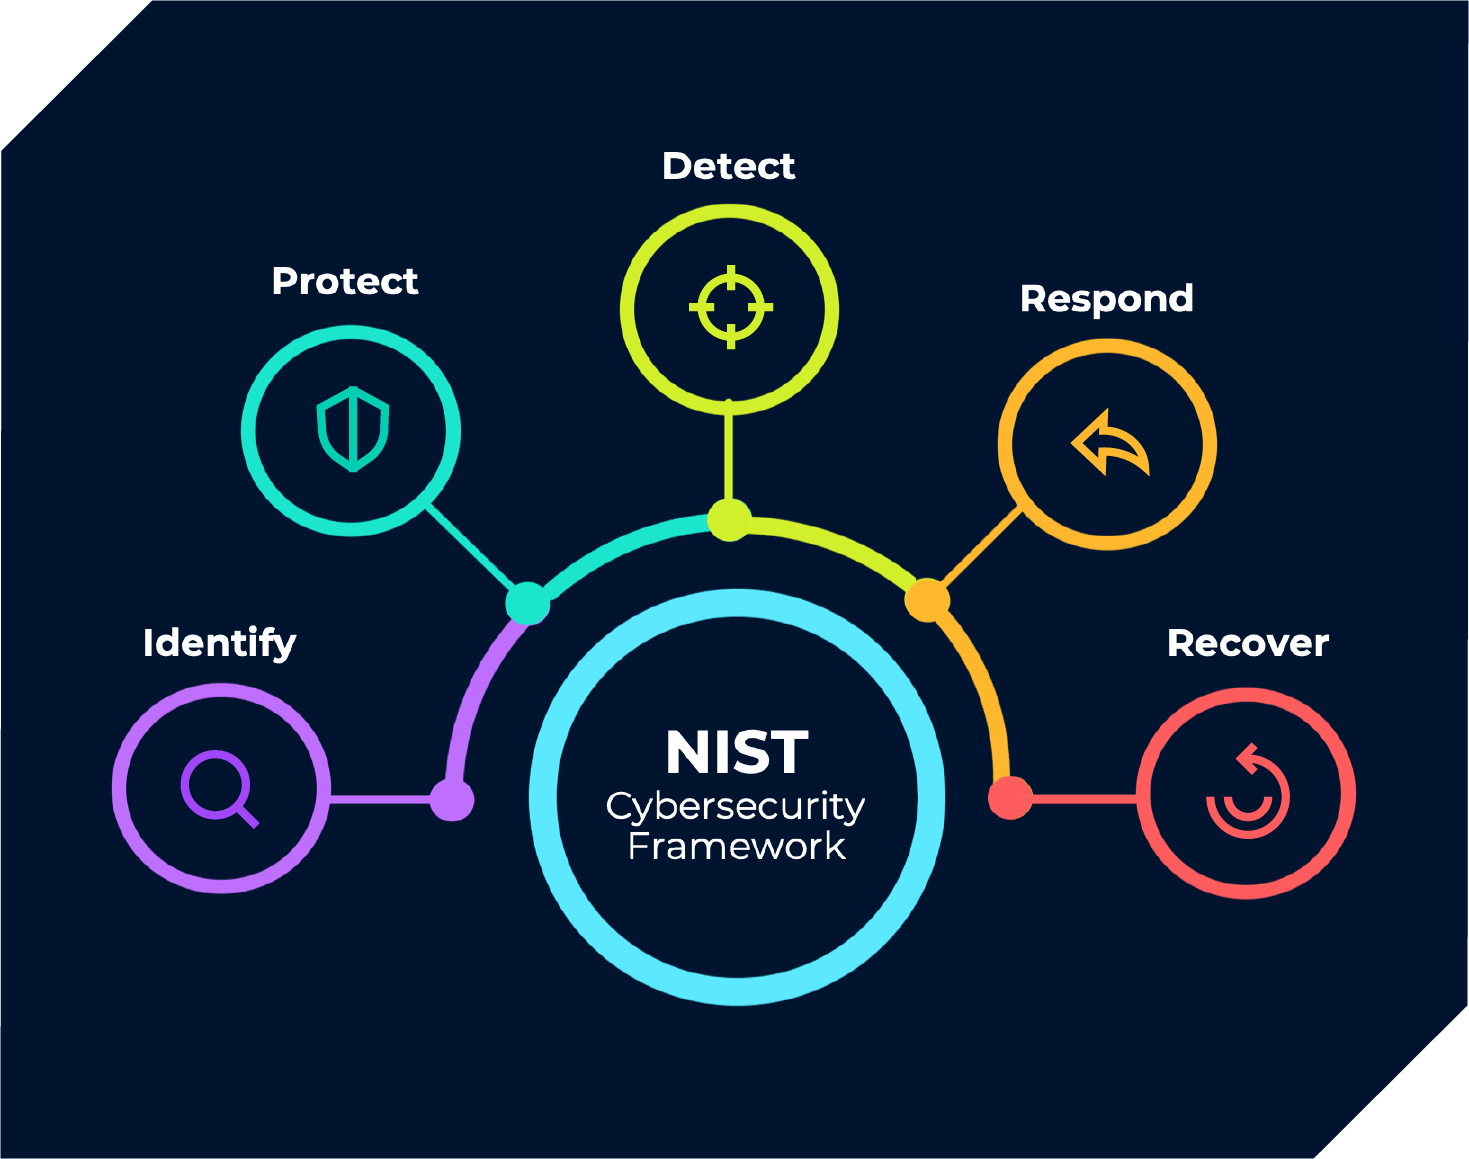
\includegraphics[width=0.8\textwidth]{Figures/qict-working-method.png}
      \caption{\acrshort{nist} working methodology that is followed by \acrshort{qict}}
\end{figure}

\begin{figure}[htbp]
      \centering
      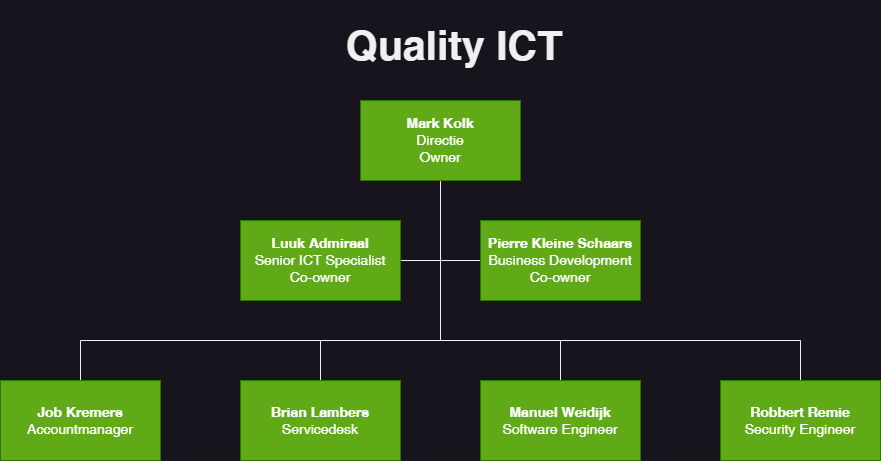
\includegraphics[width=0.8\textwidth]{Figures/OrganizationalDiagram_QICT.png}
      \caption{Flat (hierarchical) structure of \acrshort{qict}}
\end{figure}

\begin{multicols}{2}
      \section{Problem Statement}
      The company currently manages numerous third-party \acrshort{api}s for the above-mentioned purposes.
      Currently,
      Thus, the company has tasked the author with the development of the SentinelOne security threat platform integration
      for continuous cybersecurity monitoring within the \acrshort{qaas} app as the main topic of his graduation work placement
      project.

      \section{Project Objectives}
      In the end of this project which consist of 90-99 working days, the following objectives should be achieved:
      \begin{enumerate}
            \item Effectively integrates and leverages the SentinelOne \acrshort{edr} platform for continuous
                  cybersecurity monitoring within the \acrshort{qaas} app.
            \item The \acrshort{qaas} app should have a way to visualize the data retrieved from the SentinelOne
                  \acrshort{api} in a user-friendly manner in order for the client users helpdesk support, financial
                  department, cybersecurity department, software development department, and other employees within
                  \acrshort{qict}  departments to see the data easier.
            \item Combine the SentinelOne data with N-Central \acrshort{api}
            \item Utilize Vigilance package of SentinelOne
            \item Ensure proper unit testing, code refactoring, commenting, and adherence to the overall code
                  conventional guidelines and best practices in both the test and live environments of the
                  \acrshort{qaas} app.
      \end{enumerate}
      \section{Reading Guide}
      This report is structured as follows:
      \begin{itemize}
            \item \textbf{Summary}: provides a brief and concise overview of the entire report, including the
                  research questions, key findings, and conclusion. Its purpose is to provide readers with a
                  quick and comprehensive understanding of the report.
            \item \textbf{Introduction}: provides an overview of the project background, the research topic of the
                  company, and the project objectives. It introduces the context of the research and outlines the
                  structure of the report.
            \item \textbf{Research}: presents the research results, including the research methodology, the findings,
                  and the analysis of the research questions. Firstly, it describes the methodologies employed
                  during the research, and then it provides a detailed account of the research process and the
                  outcomes of the research.
            \item \textbf{Realization}: provides a detailed description of the software end-product developed during
                  this work placement project. It outlines insights into design, development, and implementation
                  phases. It also highlights key features, functionalities, and technology specifications used in
                  the project.
            \item \textbf{Conclusions and Recommendations}: the Conclusion summarizes the key findings and results
                  achieved during the research and realization phases. The Recommendation section outlines the
                  proposed next steps and future research areas to further enhance the project and address any
                  outstanding issues. It discusses potential areas for further exploration or refinement.
            \item \textbf{References}: lists all the sources cited in the report following the appropriate to
                  \acrshort{apa} 7th edition citation style.
            \item \textbf{Appendices}: includes any additional supplementary information, data, or materials that
                  are relevant to the report but not included in the main body of the report.
      \end{itemize}
\end{multicols}